\documentclass[11pt]{article}

% AMS Packages
\usepackage{amsmath} 
\usepackage{amssymb} 
\usepackage{amsthm}
% Page dimensions
\usepackage[margin=1in]{geometry}
% Images
\usepackage[pdftex]{graphicx} 
% Enumerate package
\usepackage{enumitem} 
\usepackage{array} 
% Fancify pages
\usepackage{fancyhdr} 
% Convert captions on figures to bold font
\usepackage[labelfont=bf,textfont=md]{caption}
% Time New Roman font
\usepackage{times}
% change the line spacing
\usepackage{setspace} 
% SI Units in math type
\usepackage{siunitx}
% extra symbols
\usepackage{textcomp} 
\usepackage{wrapfig}
% tikz 
\usepackage{tikz}
\usetikzlibrary{shapes.geometric, arrows}
\usepackage{bm}
% Change sizes of sections
\usepackage{titlesec}
\titleformat{\section}{\normalfont\large\bfseries}{\thesection}{1em}{}
\titleformat{\subsection}{\normalfont\bfseries}{\thesubsection}{1em}{}
\titleformat{\subsubsection}{\normalfont\small\bfseries}{\thesubsubsection}{1em}{}
% Declare useful math operators
\DeclareMathOperator*{\argmin}{arg\,min}
\DeclareMathOperator*{\plim}{plim}
\DeclareMathOperator{\Tr}{Tr}
\usepackage{float}

\usepackage{algorithm}
\usepackage[noend]{algpseudocode}
\makeatletter
\makeatother

\newcommand{\varendash}[1][5pt]{%
	\makebox[#1]{\leaders\hbox{--}\hfill\kern0pt}%
}

\pagestyle{fancy}
\chead{\textbf{\small Union of Intersections (UoI) for interpretable data driven discovery and prediction in neuroscience}}
\rhead{}
\lhead{}
\headsep 5pt

% title
\title{\textbf{Union of Intersections (UoI) for for Interpretable Data Driven Discovery and Prediction in Neuroscience}}
\author{\Large Supplementary Information}
\date{}
\begin{document}
\thispagestyle{empty}
\maketitle
\section{Coupling Models}
We applied UoI$_{\text{Lasso}}$ to coupling matrices obtained from the following datasets:
\begin{itemize}
	\item \textbf{(PVC)} Single-unit activity taken from monkey primary visual cortex (Kohn et al., 2012) in response to drifting gratings.
	\item \textbf{(A1)} Micro-electrocorticography recordings taken from rat auditory cortex (Bouchard et al., 2018) in response to tone pips.
	\item \textbf{(M1/S1)} Single-unit activity taken from monkey primary motor and somatorsensory cortices (Makin et al., 2018) during reaches on a grid of targets.
\end{itemize}

Each coupling model attempted to linearly predict the activity of a target neuron (electrode) using the activities of the remaining neurons (electrodes). We fit the coupling model with Lasso and three variants of UoI$_{\text{Lasso}}$ (optimizing for $R^2$, AIC, and BIC) through a 10-fold cross-validation. We compared the models generated by each of these variants to the model obtained via Lasso. We quantified model performance by the selection ratio (fraction of non-zero parameters), explained variance ($R^2$), Akaike Information Criterion, and the Bayesian Information Criterion. The two information criterions are defined as
\begin{align}
	\text{AIC} &= 2k - 2 \log(\hat{L}) \label{eqn:aic}\\
	\text{BIC} &= \log(n) \cdot k - 2 \log(\hat{L}) \label{eqn:bic}
\end{align}
where $\log(\hat{L})$ is the log-likelihood of the model on the test set, $n$ is the number of test samples, and $k$ is the number of features. In contrast to explained variance, lower information criterion is preferable. Thus, AIC and BIC penalize models with larger numbers of parameters (first term in equations \ref{eqn:aic} and \ref{eqn:bic}). In addition, the BIC generally prefers sparser models more strongly than the AIC.
\subsection{PVC}
This dataset was recorded by Matthew Smith and Adam Kohn and obtained through the pvc-11 dataset from CRCNS. Spiking activity was recorded from V1 in three anesthetized macaque monkeys during presentations of drifting gratings. Single-unit spiking responses were segmented into trials according to stimulus presentation. In total, there were 2400 trials recorded with 3 monkeys, each with 106, 88, and 112 single-units, respectively.

We caculated each response variable as the square-root of the spike count in the trial. Thus, the coupling model predicts whether the (square-rooted) spike count in a given trial can be described linearly by the (square-rooted) spike counts according to the remaining neurons in the population. The performance of Lasso compared to the three variants of UoI$_{\text{Lasso}}$ is depicted in Figure \ref{fig:pvc} for each monkey. We observe that UoI$_{\text{Lasso}}$ provides sparser models (top row) at limited or no cost to predictive power (second row) resulting in improved information criterion scores (bottom two rows; recall that lower information criterion is better). In addition, the three variants of UoI$_{\text{Lasso}}$ prefer different levels of sparsity, with $UoI_{\text{Lasso}}-$BIC resulting in the sparsest models.


\begin{figure}[t]
	\centering
	\scalebox{0.24}{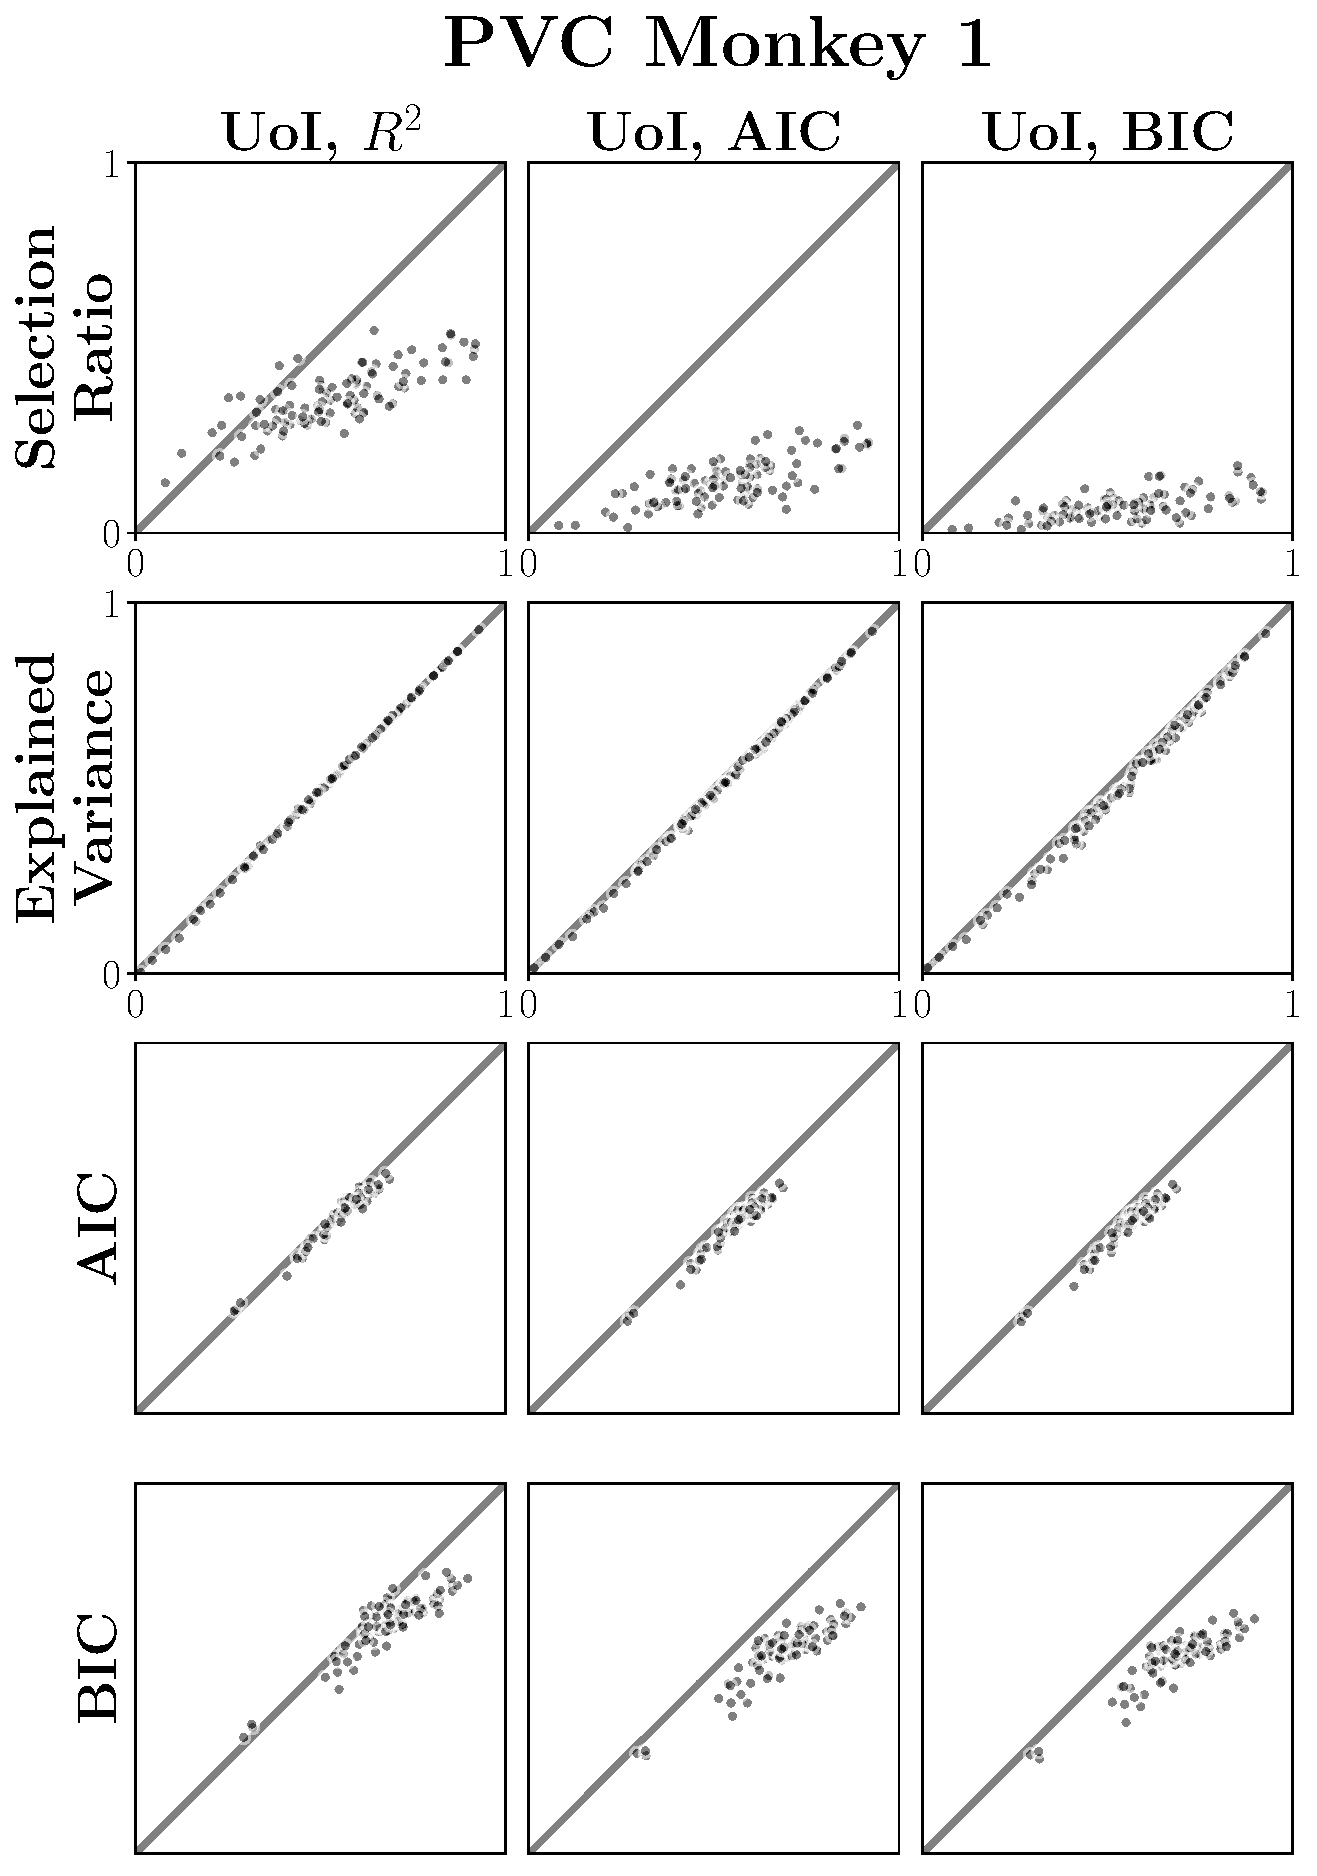
\includegraphics{img/coupling/pvc11_monkey1.pdf}}
	\scalebox{0.24}{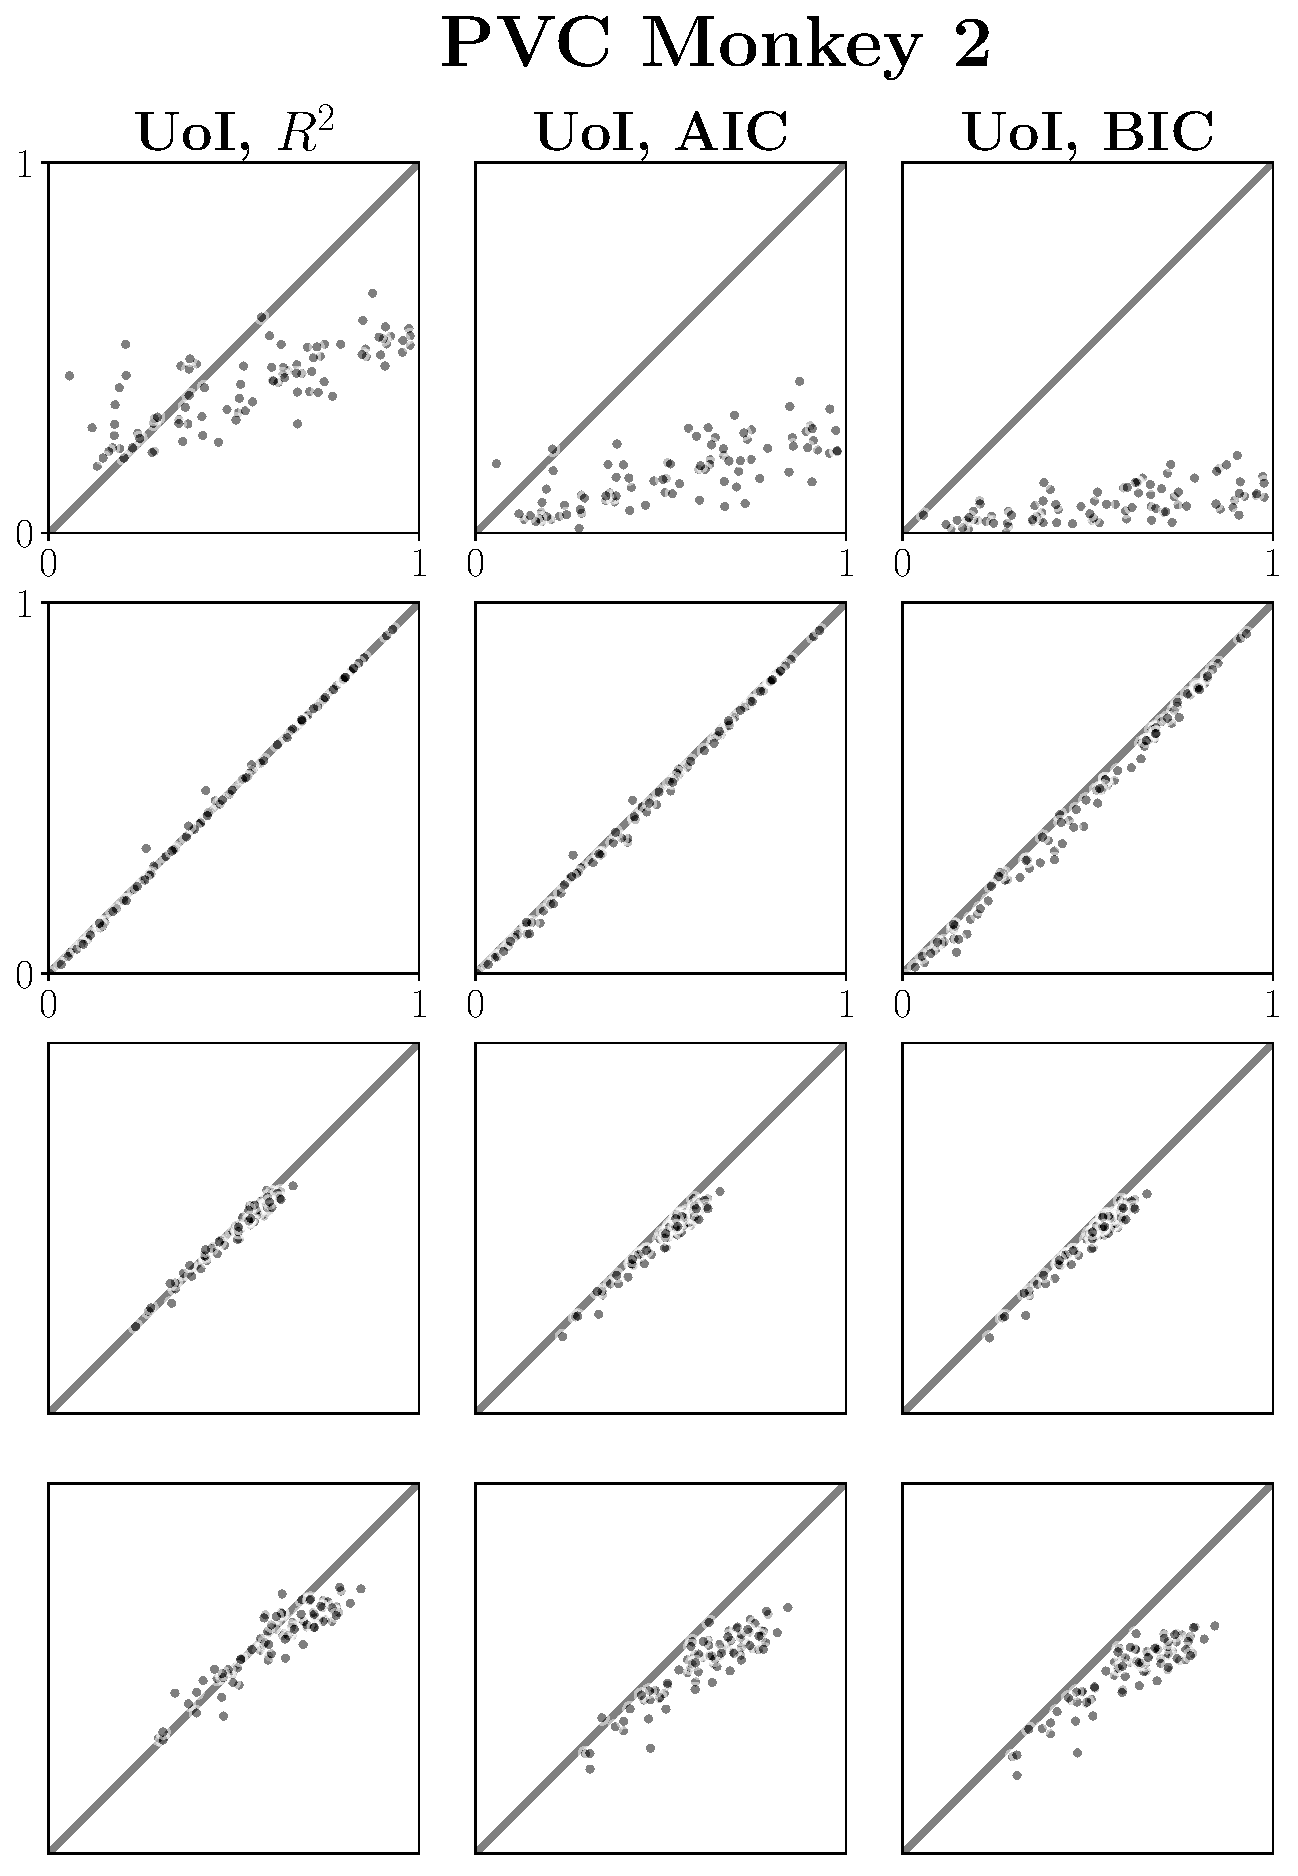
\includegraphics{img/coupling/pvc11_monkey2.pdf}}
	\scalebox{0.24}{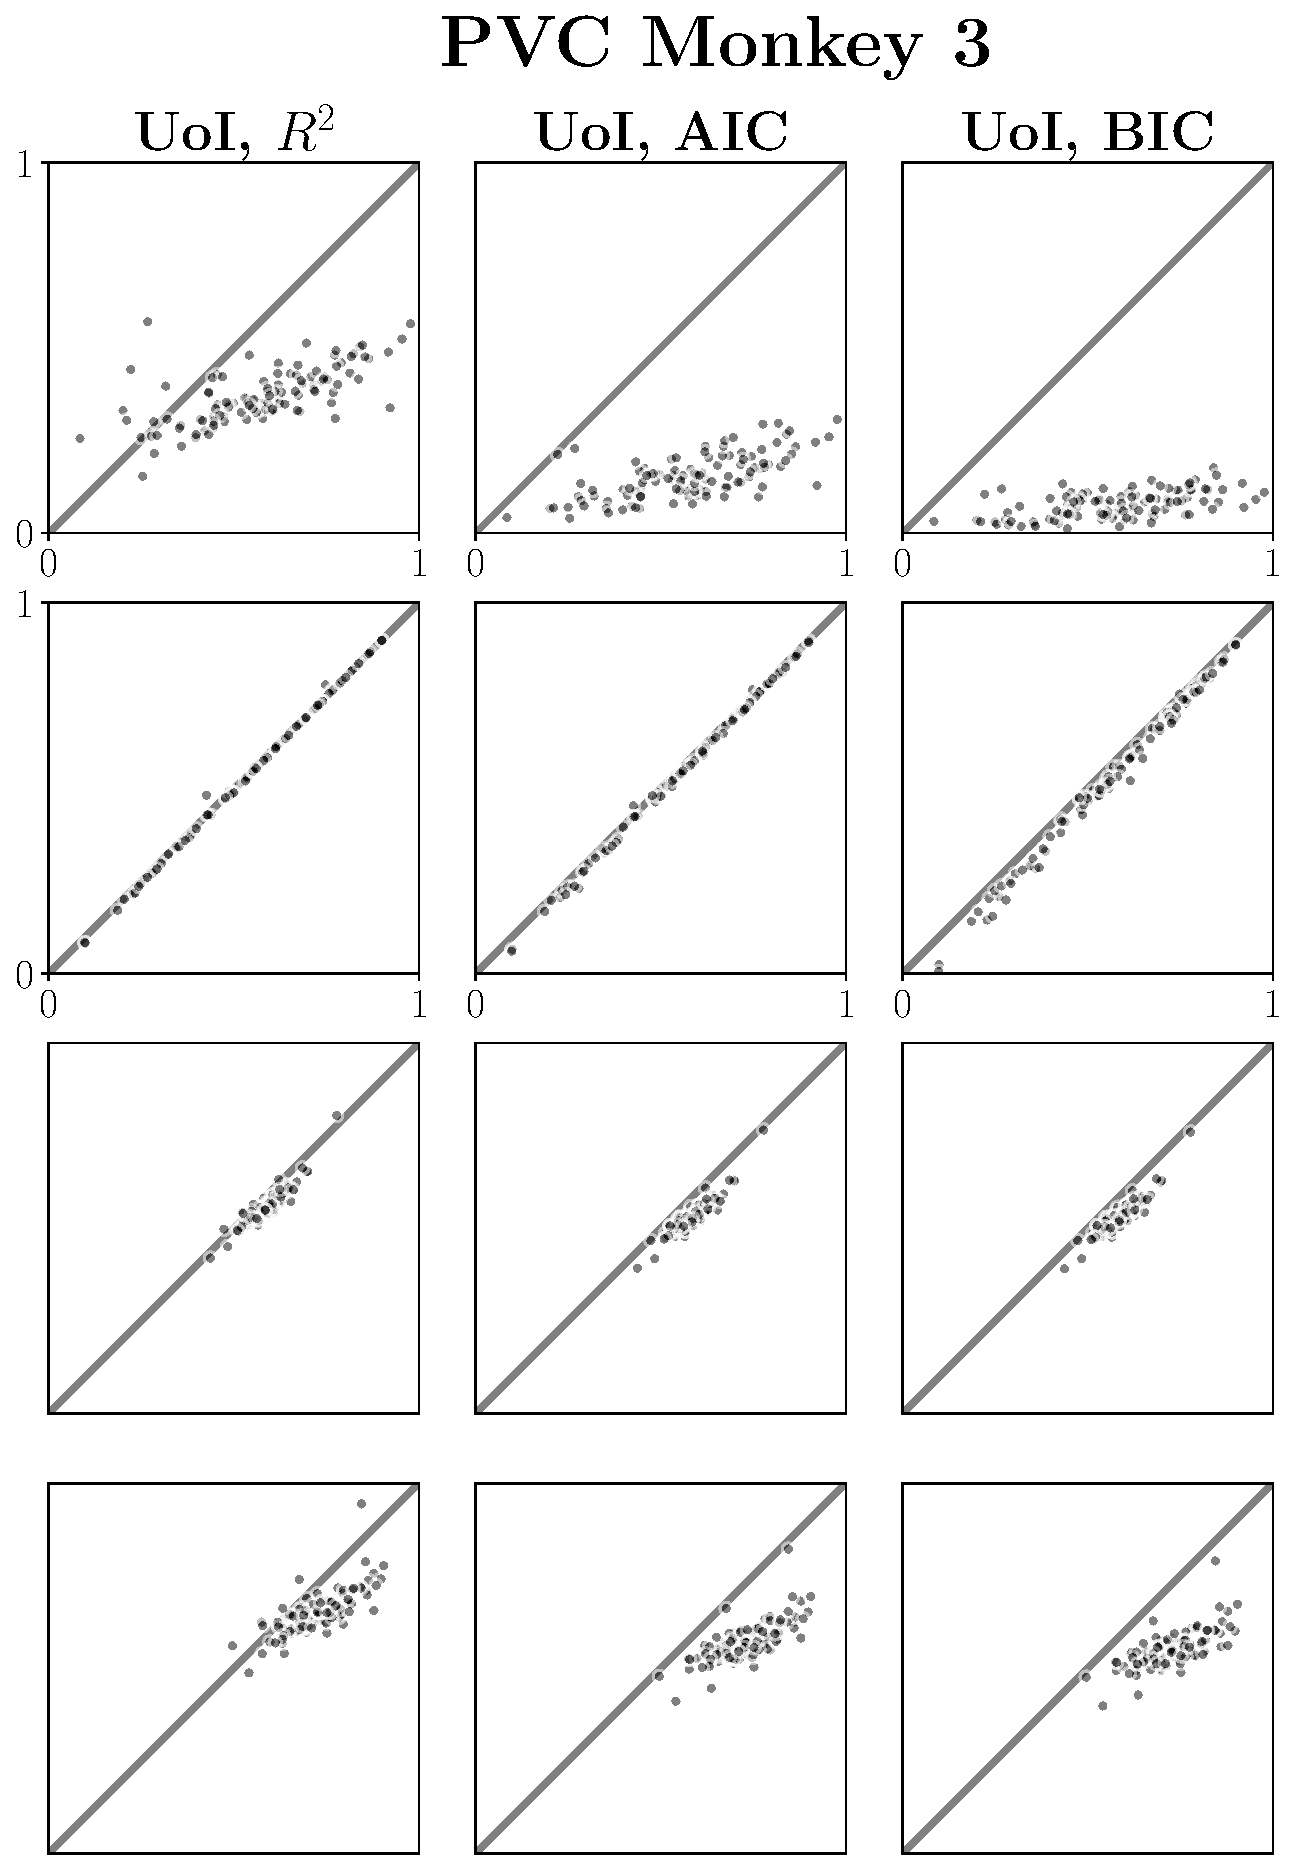
\includegraphics{img/coupling/pvc11_monkey3.pdf}}

	\caption{Lasso ($x$-axis) vs. the three variants of UoI$_{\text{Lasso}}$ ($y$-axes) on Monkey 1 (Left), Monkey 2 (Center), and Monkey 3 (Right). Metrics considered are, in order of rows, selection ratio (number of non-zero parameters divided by total possible number of parameters), explained variance ($R^2$), Akaike Information Criterion, and the Bayesian Information Criterion.}
	\label{fig:pvc}
\end{figure}


\subsection{A1}
\begin{wrapfigure}{r}{0.35\textwidth}
	\vspace{-60pt}
	\centering
	\scalebox{0.26}{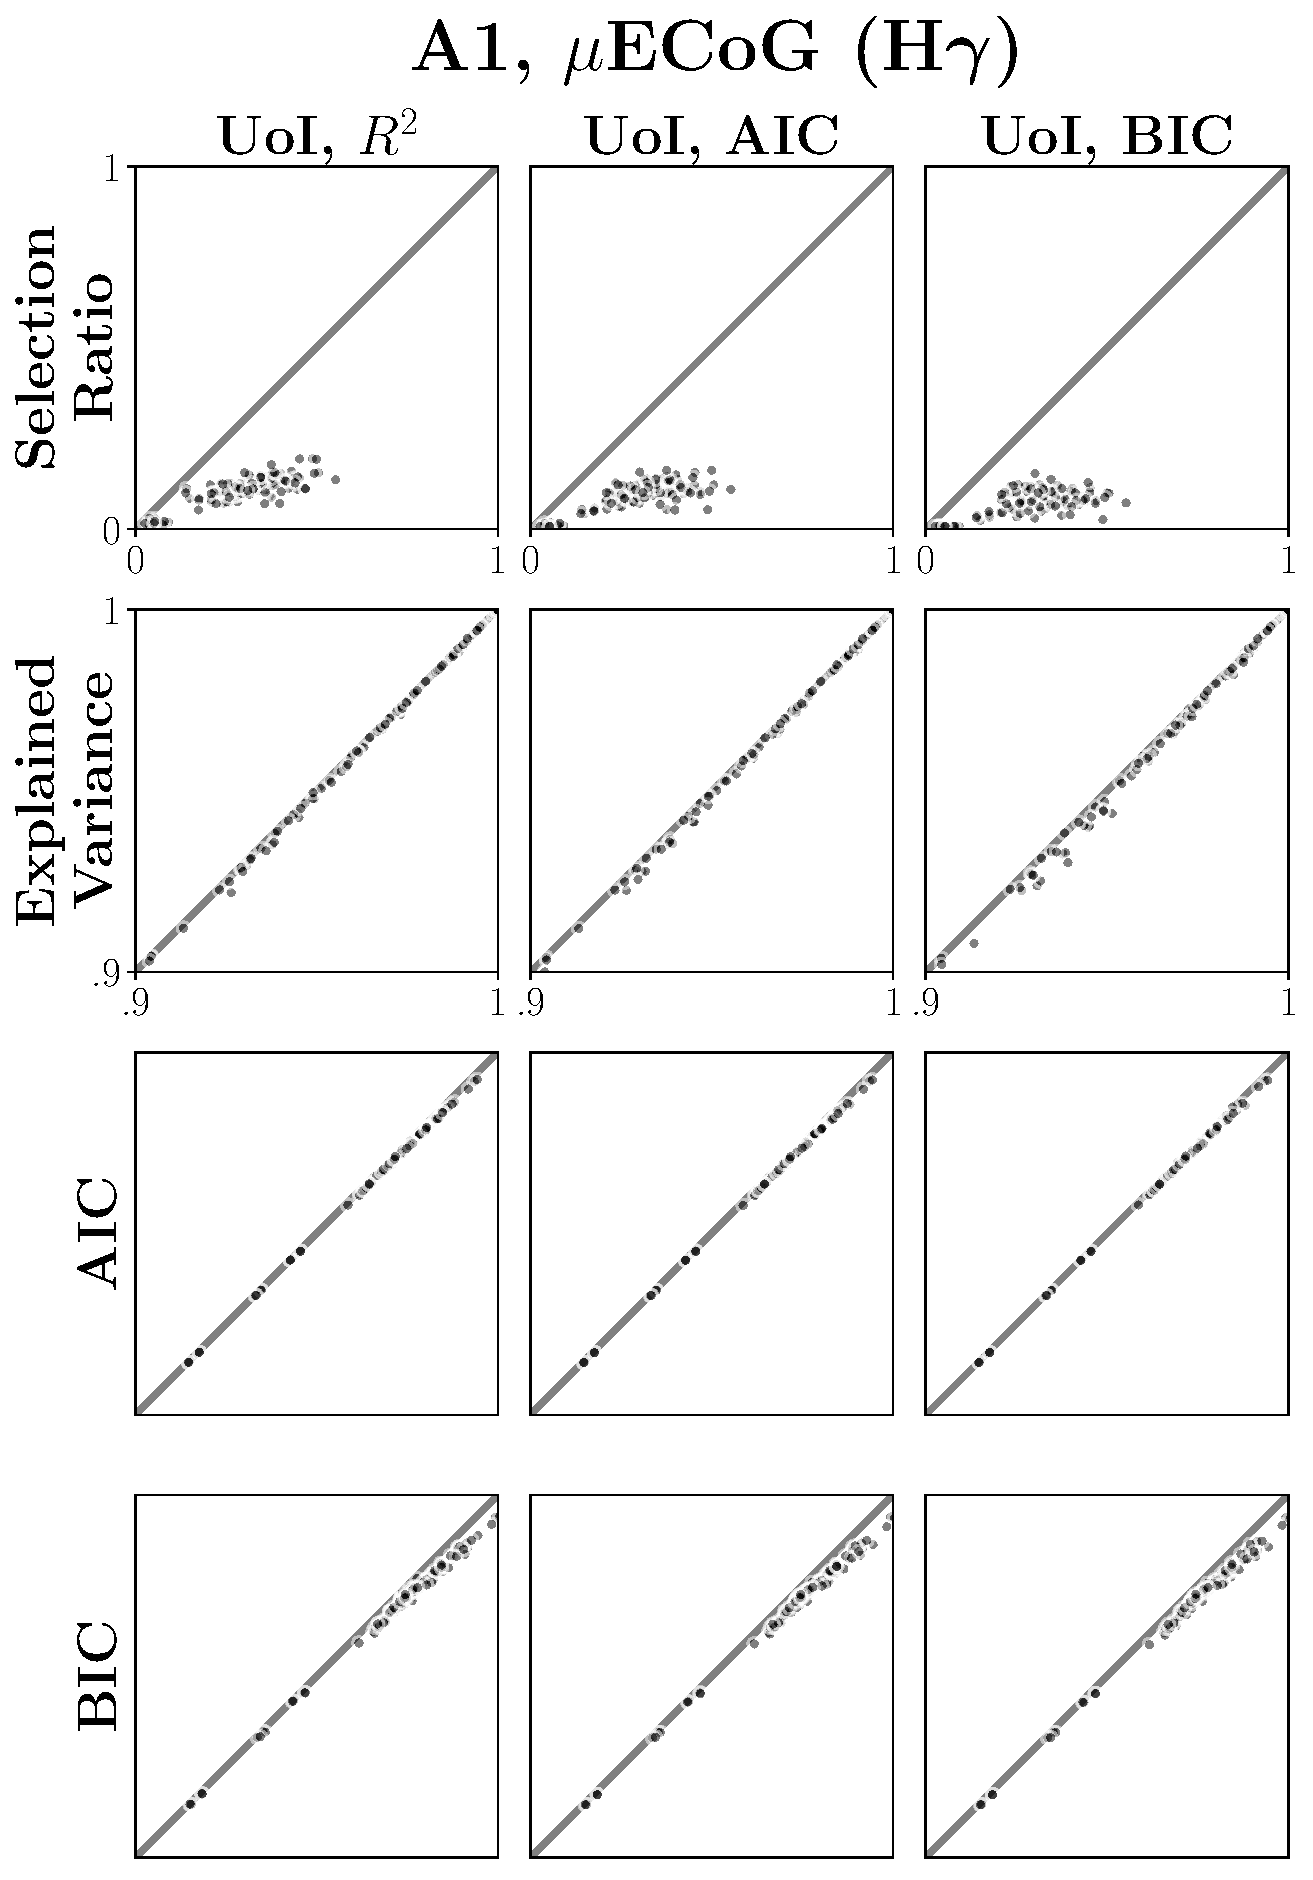
\includegraphics{img/coupling/ecog_HG.pdf}}
	\caption{Lasso ($x$-axis) vs. the three variants of UoI$_{\text{Lasso}}$ ($y$-axes) on rat auditory cortex coupling models. Rows are metrics while columns are variants of UoI$_{\text{Lasso}}$.}
	\label{fig:ecog}
\end{wrapfigure}
This dataset was recorded by the Bouchard Lab (the specific rat was R32-B7). Micro-electrocorticography was performed on the surface of the auditory cortex in anesthetized rats during the presentation of tone pips at varying frequencies and attenuations. The $\mu$ECoG recordings were  $z$-scored relative to baseline before stimulus presentation and segmented into trials based on the stimulus type. There were 4200 trials (30 frequencies, 7 attenuations, and 20 repetitions) and 128 electrodes. 

We calculated each response variable as the peak response of the $z$-scored high-gamma analytic amplitude. Thus, the coupling model predicts whether the peak response in a given trial can be described linearly by the peak responses of the remaining electrodes. A comparison of Lasso to the variants of UoI$_{\text{Lasso}}$ are shown in Figure \ref{fig:ecog}. Note that the explained variance plots cover the range $[0.9, 1.0]$, since the coupling models were highly predictive. UoI$_{\text{Lasso}}$ resulted in considerably sparser models coming at little to no cost to explained variance.  Similarly to the previous Figure, we observe that there is a spectrum of enforced sparsity, with UoI$_{\text{Lasso}}$--BIC providing the sparsest models. For this dataset, UoI$_{\text{Lasso}}$--AIC provides a good balance between sparsity and predictive power.

\subsection{M1}
\begin{wrapfigure}{r}{0.35\textwidth}
	\vspace{-25pt}
	\centering
	\scalebox{0.26}{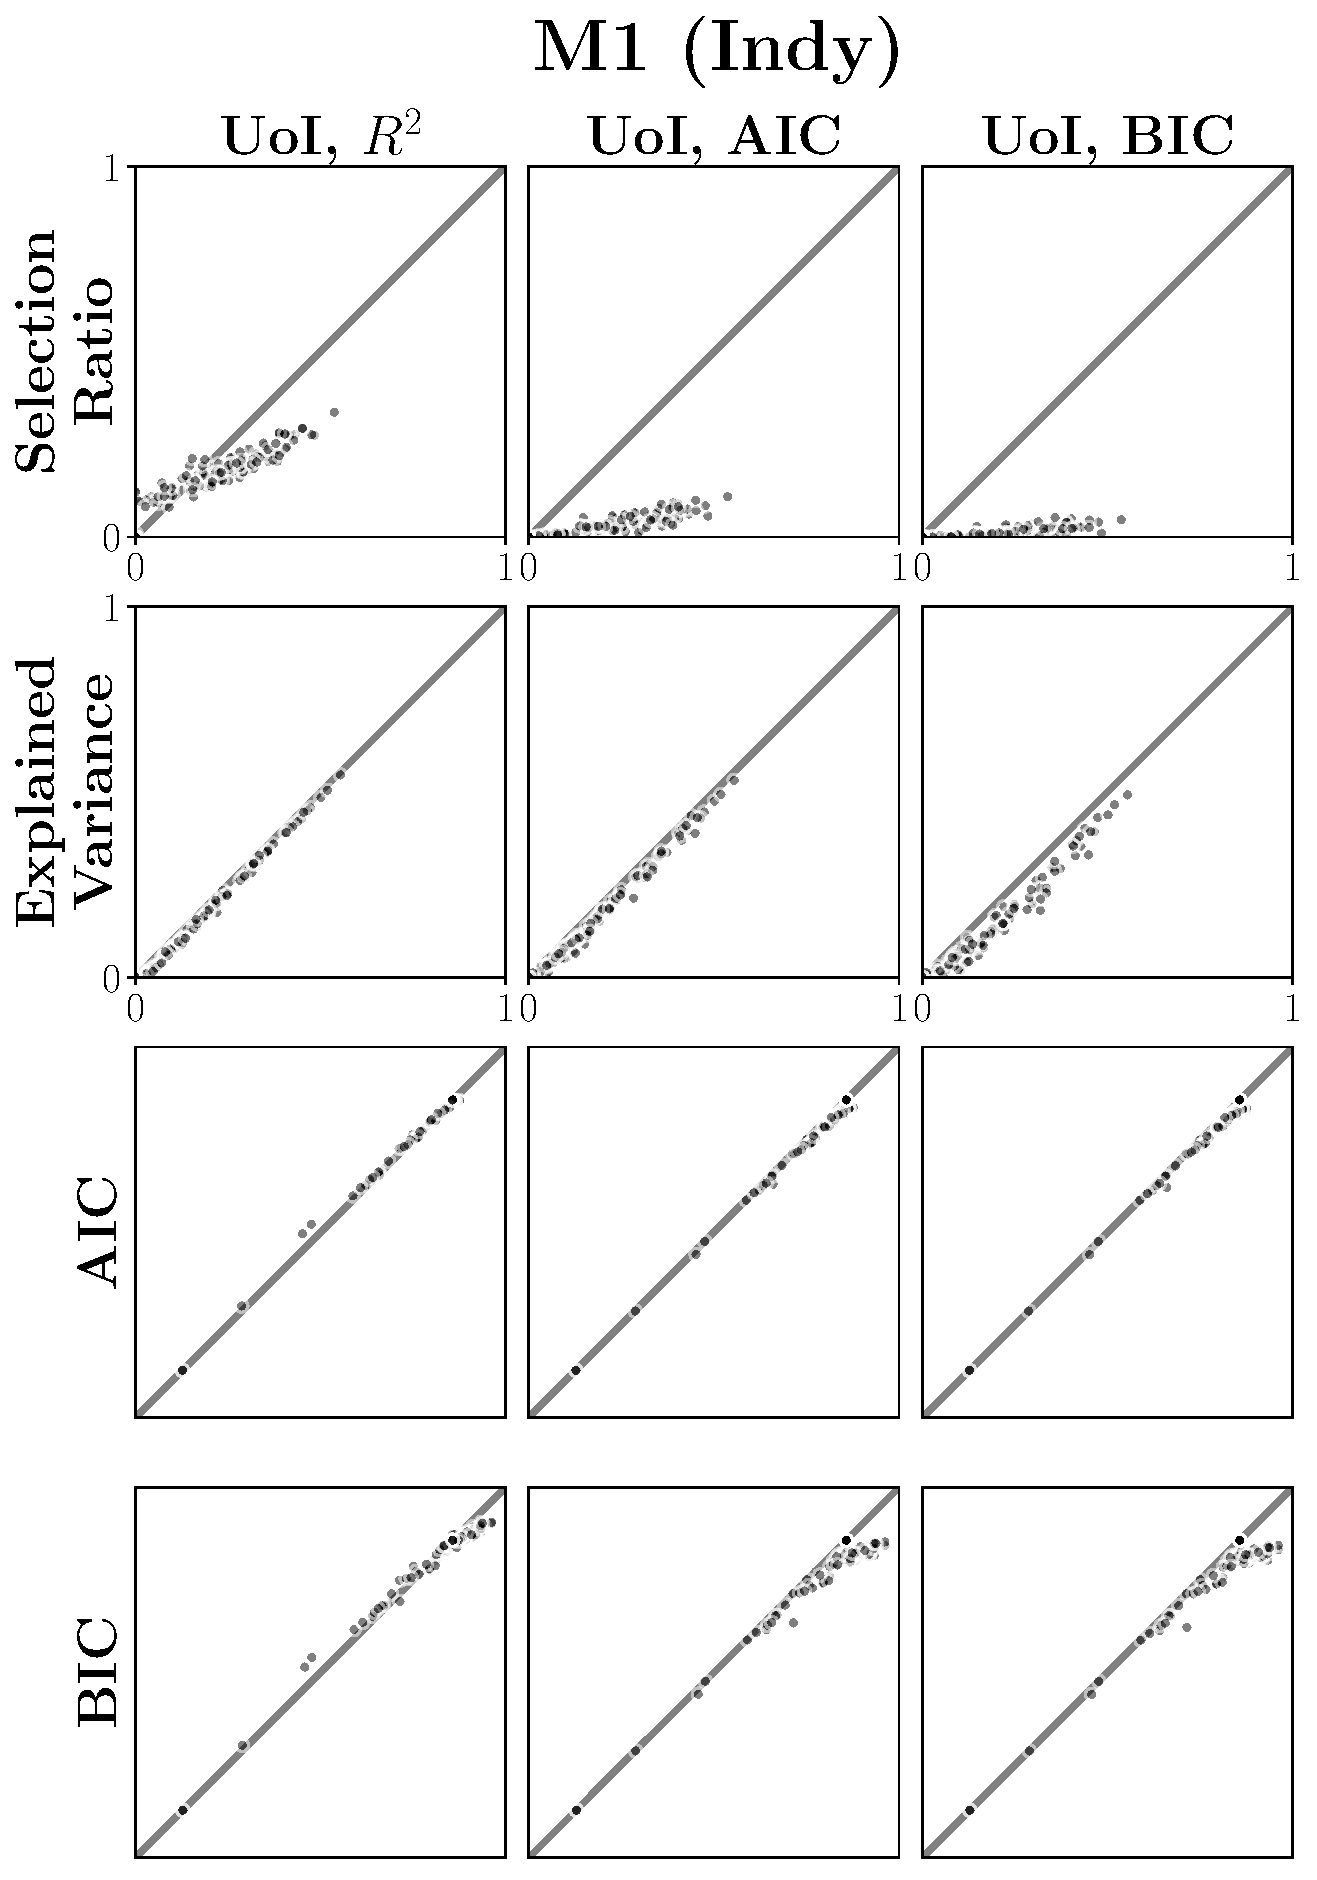
\includegraphics{img/coupling/nhp_indy_20160411_01.pdf}}
	\caption{Lasso ($x$-axis) vs. the three variants of UoI$_{\text{Lasso}}$ ($y$-axes) on nonhuman primate coupling models.}
	\label{fig:nhp}
\end{wrapfigure}
This dataset was recorded by the Sabes Lab (obtained through Zenodo). Single-unit responses were obtained from non-human primate primary motor cortex during self-paced reaches to target on a grid. The primate was prompted to reach for a specific target without gaps or pre-movement delay intervals. We binned the total spike trains for all the recorded single-units to widths of 500 milliseconds. According to this binning, there were 1716 samples for 196 single-units.

We caculated each response variable as the square-root of the spike count in the bin. Thus, the coupling model predicts whether the (square-rooted) spike count in a given bin can be described linearly by the (square-rooted) spike counts according to the remaining neurons in the population. 

The performance of Lasso compared to the three variants of UoI$_{\text{Lasso}}$ is depicted in Figure \ref{fig:nhp} for a given primate (Indy) and session (04-11-2016-1). Interestingly, UoI$_{\text{Lasso}}$ provides sparser models except for a subset of neurons under the UoI$_{\text{Lasso}}-R^2$ variant. However, UoI$_{\text{Lasso}}$ still maintains predictive performance, resulting in simpler but predictive models.\\

\newpage

\section{Tuning}
\subsection{A1}

\begin{wrapfigure}{r}{0.35\textwidth}
	\vspace{-40pt}
	\centering
	\scalebox{0.26}{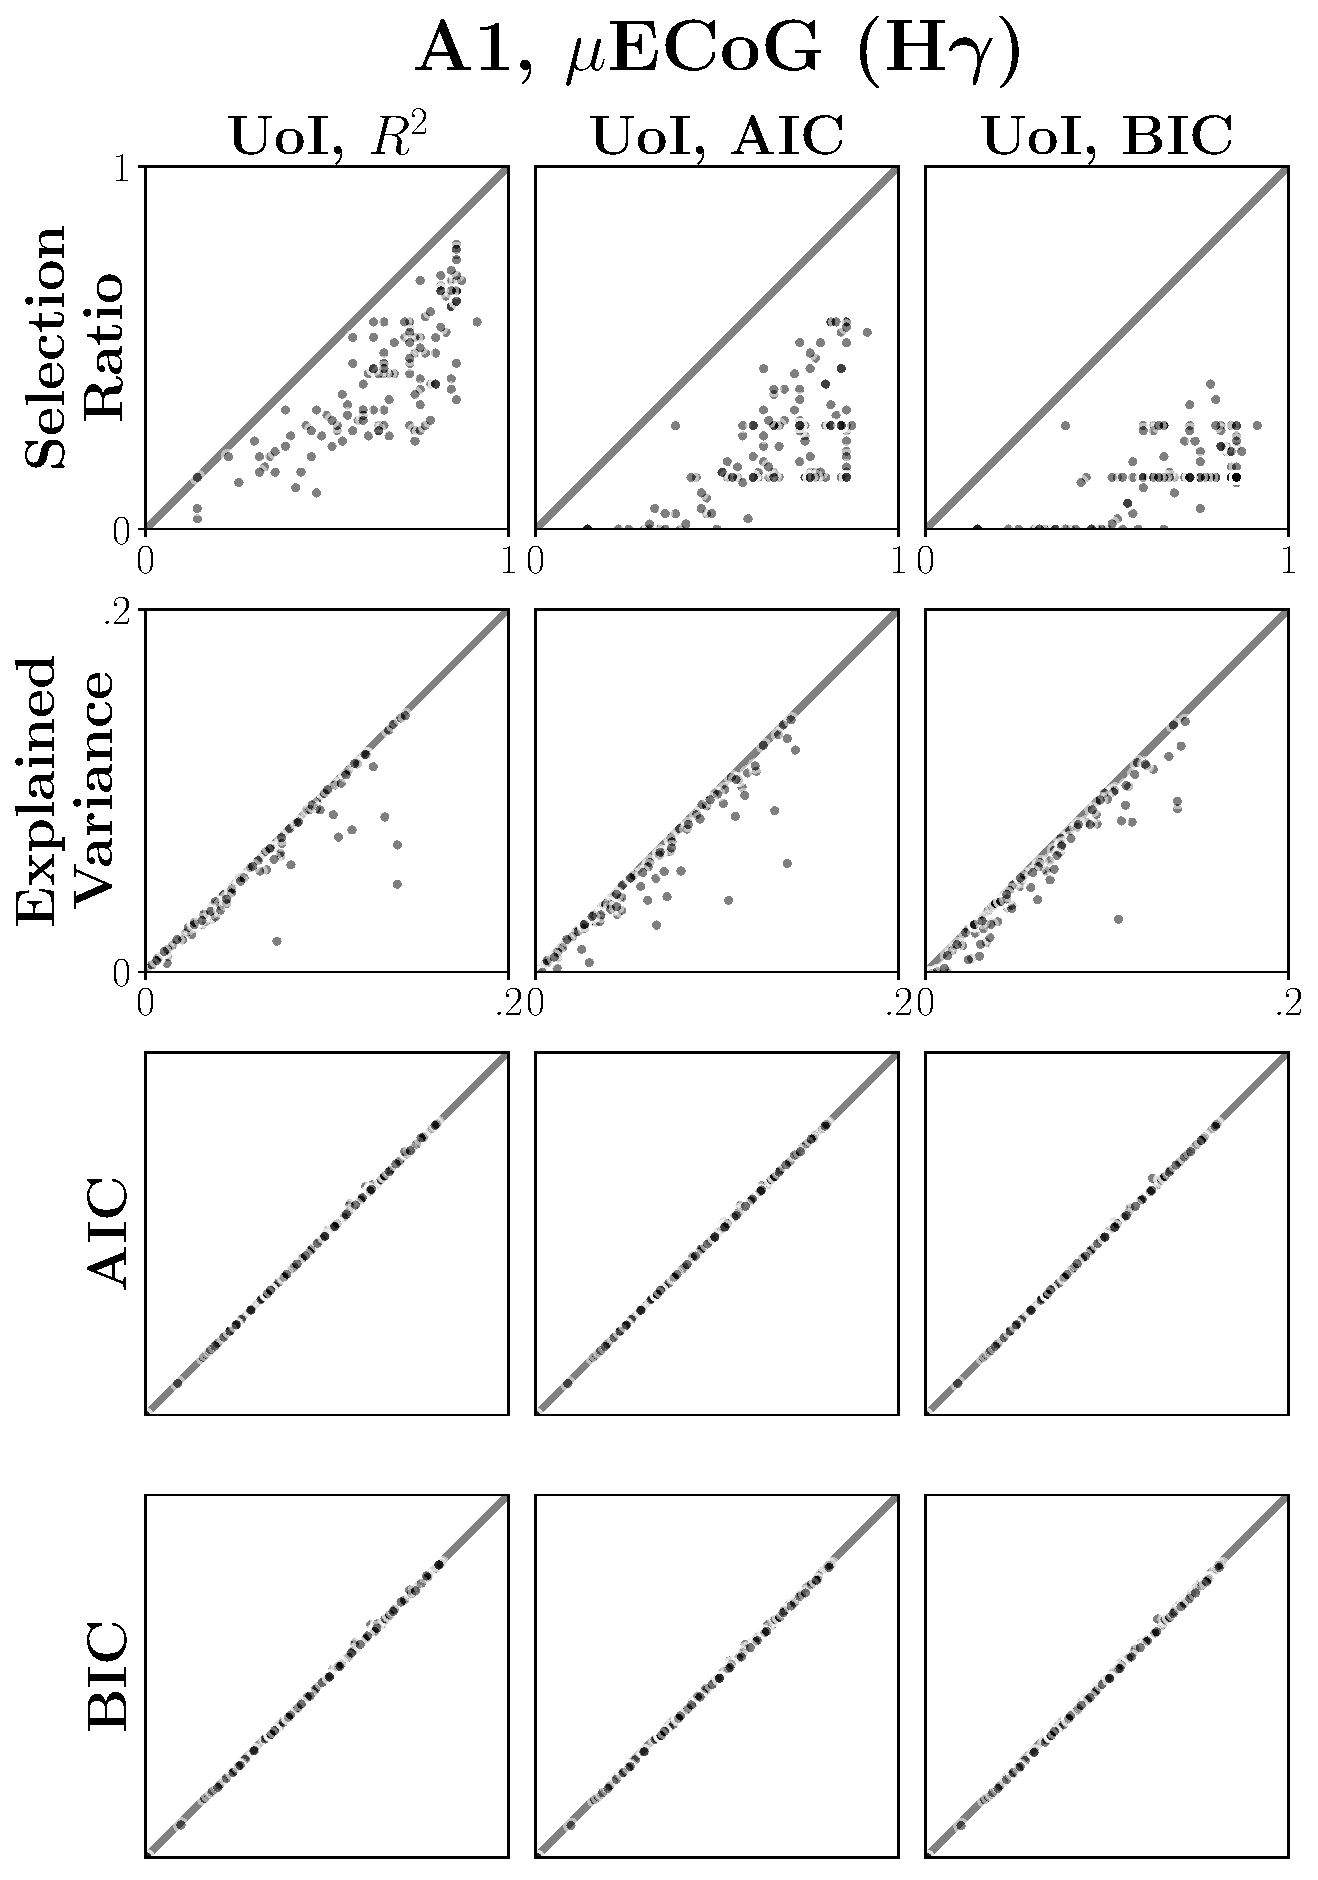
\includegraphics{img/tuning/ecog_hg.pdf}}
	\caption{Lasso ($x$-axis) vs. the three variants of UoI$_{\text{Lasso}}$ ($y$-axes) for auditory tuning data.}
	\label{fig:ecog_tuning_scores}
	\vspace{-30pt}
\end{wrapfigure}
We fit tuning curves to the auditory $\mu$ECoG recordings using Gaussian basis functions tiling the log-frequency axis. Specifically, the response $y_i$ for a given electrode was modeled as
\begin{align}
y_i(f) &= a_0 + \sum_{j=1}^k a_j \exp\left(-\frac{(f - f_j)^2}{2\sigma_i^2}\right)
\end{align}
where $f_j$ are spread evenly in log-frequency, $k$ is the number of Gaussians (features), and $\sigma_i$ is the spread of the Gaussian basis functions, generally chosen uniformly across all electrodes. The relevant tuning parameters to be fit are the $a_j$. For the $\mu$-ECoG data, we used 7 Gaussians spread evenly from  0.5 to 32 kHz, and $\sigma_i^2=0.64$ octaves. We fit this model using Lasso and the UoI$_{\text{Lasso}}$ variants.

The model performance is shown in Figure \ref{fig:ecog_tuning_scores}. Note that the maximum number of features that can be used is 7, so differences in selection ratio denote a difference in only a few features. In this case, UoI$_{\text{Lasso}}-R^2$ uses fewer features to achieve the same predictive performance for almost all electrodes. There is little different in the information criteria because the number of features is small compared to the amount of data.

In addition, we also examined tuning curves across the $\mu$ECoG grid. The curves are shown in Figure \ref{fig:ecog_tuning_curves}, plotted against log-frequency. Lasso and UoI$_{\text{Lasso}}$ generally agree on almost all electrodes. Both fitting procedures result in broad tonotopy across the grid. For some electrodes, UoI$_{\text{Lasso}}-$BIC (dashed red) zeros out all coefficients except the intercept. In these cases, the penalty for requiring parameters is greater than the relatively weak model performance (observe the scale in Figure \ref{fig:ecog_tuning_scores}).
\begin{figure}[b!]
	\centering
	\scalebox{0.435}{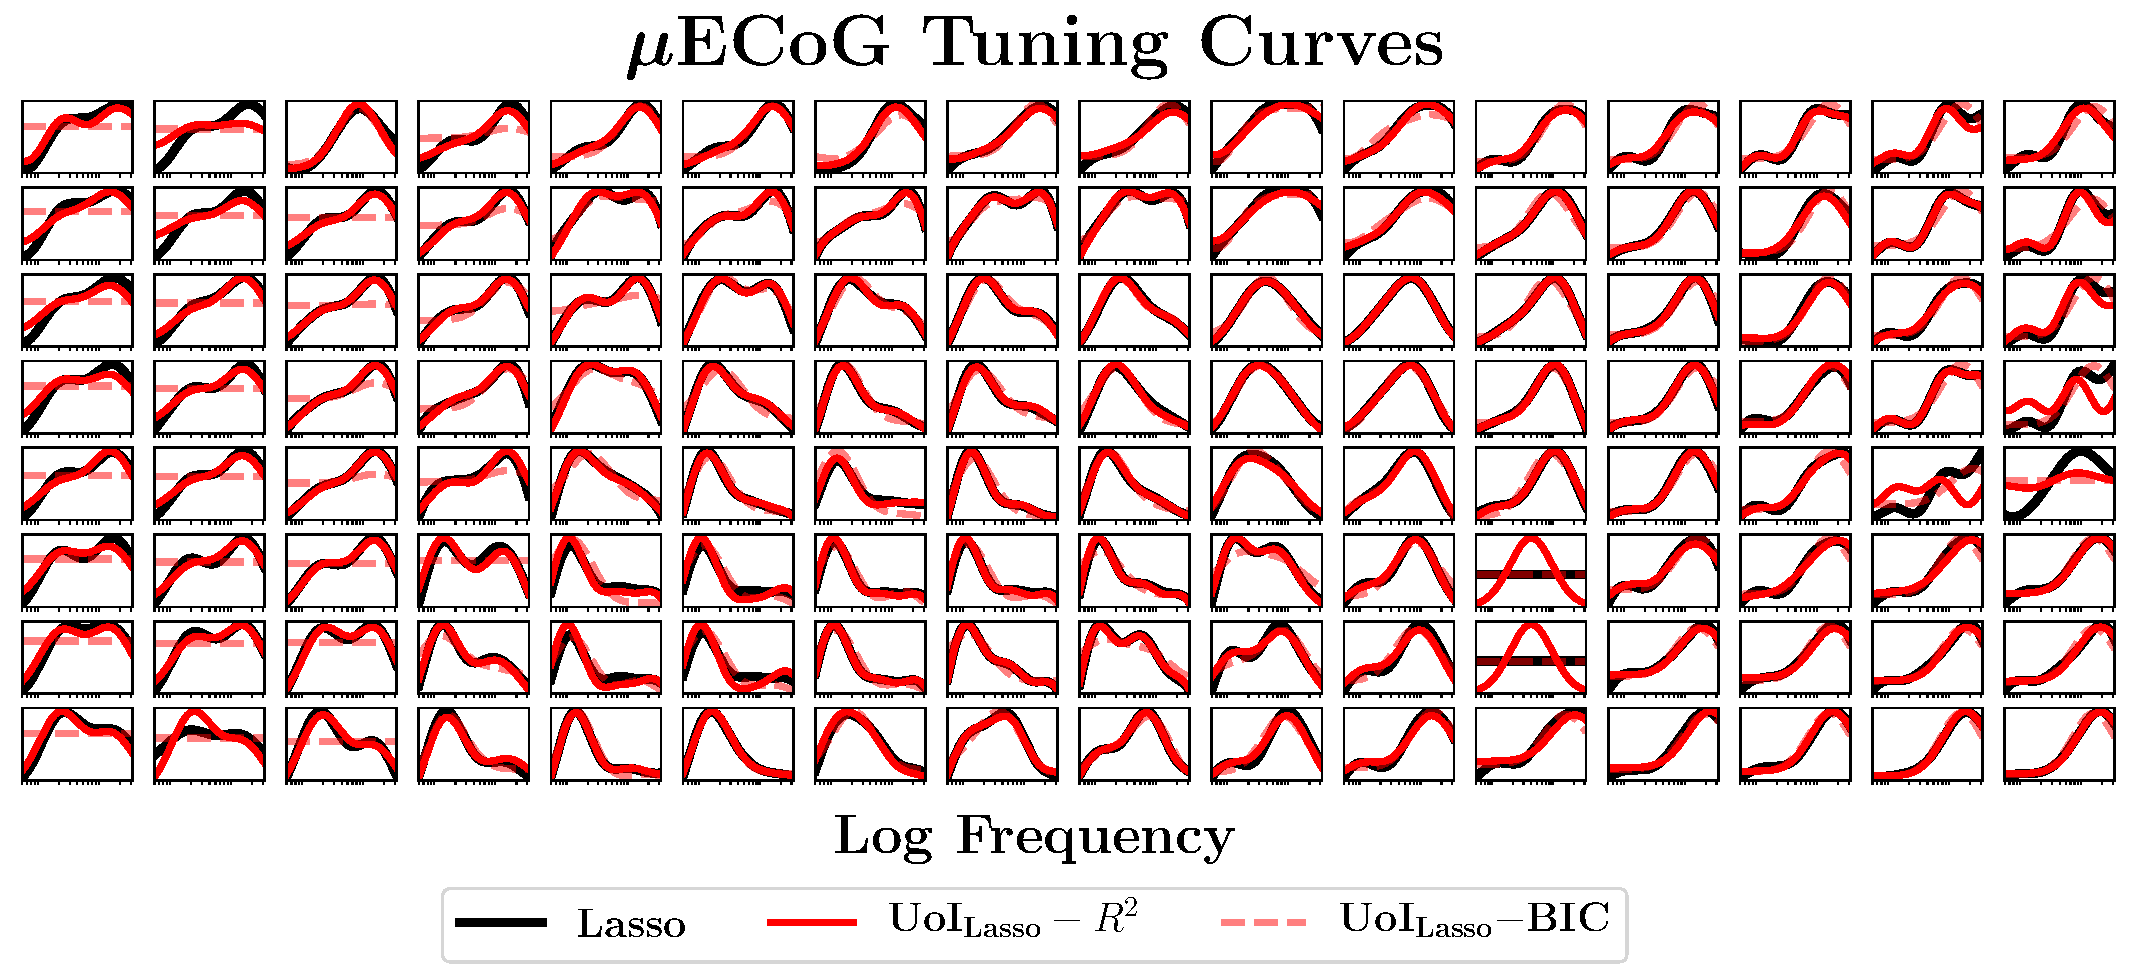
\includegraphics{img/tuning/ecog_grid.pdf}}

	\caption{Auditory tuning curves plotted against log-frequency for each electrode on the $\mu$ECoG grid. Three separate fits are shown: Lasso (black), UoI$_{\text{Lasso}}-R^2$ (red) and UoI$_{\text{Lasso}}-$BIC (dashed red).}
	\label{fig:ecog_tuning_curves}
\end{figure}

\subsection{Retina}

We fit spatio-temporal receptive fields to retinal data on data obtained by the Meister lab. This stimulus in this dataset consists of random bars (ON/OFF) flashed to isolated retinal ganglion cells from mice. Since the data is effectively one-dimensional, the resulting STRFs will be one-dimensional in space. We calculated STRFs by performing spike-triggered averaging for different delays (sweeping over some predetermined window length). The resulting fitted coefficients can be visualized on a plot with time on one axis and space on the other.

We fit STRFs to 10 different recordings. An example STRF (comparing Lasso to UoI$_{\text{Lasso}}$)  along with statistics across the 10 fits is shown in Figure \ref{fig:strfs} below. We observe that the STRFs generated by UoI$_{\text{Lasso}}$ are much sparser and cleaner. Features that are extraneous for predicting the neural responses are removed when applying UoI$_{\text{Lasso}}$. This is quantified by the selection ratio and change in $R^2$ (specifically, change in $R^2$ from baseline to peak):  Figure \ref{fig:strfs}, right. We note that we used the AIC estimation score, which offered the best balance between choosing models that were predictive but also sparse. While the $R^2$ estimation score also worked well, the resulting STRFs did not look at clean.

\begin{figure}[h!]
	\centering
	\scalebox{1}{\includegraphics{img/tuning/example_strf.pdf}}
	\scalebox{1}{\includegraphics{img/tuning/strf_statistics.pdf}}
	
	\caption{\textbf{Left:} comparison of STRFs obtained by using Lasso and UoI$_{\text{Lasso}}$ to regularize the spike-triggered averaging. \textbf{Right:} Top, selection ratio comparison across 10 fits. Bottom, the change in $R^2$ from baseline to peak over the window length.}
	\label{fig:strfs}
\end{figure}

\newpage 
\section{Classification}
\subsection{Recordings from Basal Ganglia}
We consider a dataset from the Berke lab involving recordings from the basal ganglia of rats. Specifically, these datasets are taken from the  globus pallidus (GP) and substantia nigra pars reticulata (SNr). These regions generally participate in race pathways during decision making. The task that allowed the experimenters to assess these pathways is as follows:
\begin{itemize}
	\item A rat is prompted to enter its head in one of three ports using a visual cue. 
	\item Once the rat has placed its head through the port, it is then prompted, with a tone, to either go to the left port or right port. The frequency of the tone indicates whether it should be left or right (GO condition).
	\item On some fraction of the trials, the direction tone will be followed by a white noise burst, indicating that the rat should remain in the center port (STOP condition).
	\item In some trials, the rat moves before the GO tone occurs, which is considered a pre-tone failure.
\end{itemize}
Thus, there are several decisions that can be predicted based on the neural recordings. Can we:
\begin{itemize}
	\item Predict whether the rat made a pre-tone error according to the neural activity? (432 trials).
	\item Predict whether the trial was a GO or STOP trial based on the neural activity? (326 trials).
	\item Predict whether the trial was a left or right GO trial based on the neural activity? (186 trials).
\end{itemize}

\subsection{Prediction of pre-tone failure}
We used neural activity to predict whether a rat would fail on a trial pre-tone. Specifically, we examined spike counts of the 18 units in GP  and 36 units in SNr in a timespan following the point when the rat enters the center port. On pre-tone failures and successes, the rat typically had different time lengths between the center-in and center-out (Figure \ref{fig:delays}, left). 

\begin{figure}[b]
	\centering
	\includegraphics[scale=0.265]{img/classification/delay_distribution_pretone.pdf}
	\includegraphics[scale=0.265]{img/classification/delay_distribution_lr.pdf}
	\includegraphics[scale=0.265]{img/classification/delay_distribution_sg.pdf}
	\caption{\textbf{Left:} Time between center-in and center-out for pre-tone failures (red) and successes (blue). \textbf{Middle:} Time between side-cue event and center-out on left (black) and right (red) trials. \textbf{Right:} Time between side-cue event and center-out on stop (black) and go (red) trials.}
	\label{fig:delays}
\end{figure}

First, we examined firing rates of the neurons in GP and SNr. We applied a Gaussian kernel to the spike times with sampling rate 500 Hz and variance 0.075 seconds$^2$ in the window $(C_0, C_0 + \Delta t)$. The firing rates for the GP and SNr neurons are depicted in Figures \ref{fig:gp_pretone} and \ref{fig:snr_pretone}. Among both populations, there are clearly neurons that are not very active, neurons that are highly active but not distinguishable between the two trial conditions, and neurons that are very active and distinguishable between the two trial conditions. Thus, this neural population is suitable for decoding.

\begin{figure}[H]
	\centering
	\includegraphics[scale=0.43]{img/classification/gp_pretone_fr.pdf}
	\includegraphics[scale=0.45]{img/classification/gp_pretone_fits.pdf}
	\caption{\textbf{Top:} Firing rates for GP neurons in the 0.5 second window after center-in. Thin curves denote individual trials, while thick curves denote trial averages. Red curves refer to pre-tone failures while black curves refer to pre-tone successes. \textbf{Bottom:} Logistic regression (top) and UoI$_{\text{Logistic}}$ fits on models predicting pre-tone success/failure using spike counts in the $(C_0, C_0+\Delta t)$ window. Location on grid refers to neuron in top of plot. Features selected out are denoted by and `x'.}
	\label{fig:gp_pretone}
\end{figure}

\begin{figure}[H]
	\centering
	\includegraphics[scale=0.34]{img/classification/snr_pretone_fr.pdf}
	\includegraphics[scale=0.35]{img/classification/snr_pretone_fits.pdf}
	\caption{\textbf{Left:} Firing rates for SNr neurons in the 0.5 second window after center-in. Thin curves denote individual trials, while thick curves denote trial averages. Red curves refer to pre-tone failures while black curves refer to pre-tone successes. \textbf{Right:} Logistic regression (top) and UoI$_{\text{Logistic}}$ fits on models predicting pre-tone success/failure using spike counts in the $(C_0, C_0+\Delta t)$ window. Location on grid refers to neuron in top of plot. Features selected out are denoted by and `x'.}
	\label{fig:snr_pretone}
\end{figure}
\begin{figure}[H]
	\centering
	\includegraphics[scale=0.49]{img/classification/pretone_metrics.pdf}
	\caption{Accuracy (left) and selection ratio (right) for GP and SNr populations across the five folds.}
	\label{fig:pretone_metrics}
\end{figure}

We applied Logistic Regression and UoI$_{\text{Logistic}}$ with an accuracy estimation score to predict the trial condition given the spike counts in the window $(C_0, C_0 + \Delta t)$. We performed fits separately for GP and SNr neurons using 5-fold cross-validation. The resulting fits (calculated as a median across folds) are depicted in Figures \ref{fig:gp_pretone} and \ref{fig:snr_pretone} in a grid that matches the firing rate grid. Generally:
\begin{itemize}
	\item UoI$_{\text{Logistic}}$ exhibits much sparser fits.
	\item These sparser fits come at no cost to predictive accuracy.
	\item These fits correspond to neurons that generally observe different firing patterns for the pre-tone failure and pre-tone success conditions.
\end{itemize}

The first two observations are summarized by the selection ratio and accuracy, plotted for the GP and SNr populations in Figure \ref{fig:pretone_metrics}, where we plot the accuracy on the validation sets (5 points) and the selection ratios of the 5 fits. The accuracy is benchmarked to chance, which is roughly 75\%, because three-quarters of the trials are pre-tone successes.

\subsection{Prediction of left-right trials}
Next, we used neural activity to predict whether a rat went left or right on successful GO trials. Specifically, we examined spike counts of the 18 units in GP  and 36 units in SNr in a timespan following the point when the side-cue tone occurs. The time length between side-cue tone events and center-out events were generally the same across left/right GO trials (Figure \ref{fig:delays}, middle). There were more successful left trials (106) than successful right trials (80).

We considered the window $(T_0, T_0 + \Delta t)$ where $T_0$ is the side-cue event time and $\Delta t$ is 0.5 seconds (i.e. on most trials, the rat has left the center port in this window). As before, we plot the firing rates for the GP and SNr neurons in this window (with the same Gaussian kernel) in Figures \ref{fig:gp_posttone} and \ref{fig:snr_posttone}. Furthermore, we fit classifiers in the same fashion as the previous subsection and plot the median coefficients in the same figures. Our conclusions are:
\begin{itemize}
	\item  UoI$_{\text{Logistic}}$ exhibits much sparser fits for GP. These sparser fits come at no cost to predictive accuracy.
	\item UoI$_{\text{Logistic}}$ exhibits the same degree of sparsity for the SNr neurons. The resulting fits imply that two neurons are highly predictive of left/right trials. Specifically, if these neurons fire, the trial is highly likely to be a successful right trial. 
	\item In the SNr fits, UoI$_{\text{Logistic}}$ provides fitted values that are an order of magnitude larger than regularized Logistic regression.
\end{itemize}
In Figure \ref{fig:posttone_metrics}, we observe the above conclusions quantified. Note that for SNr, we obtained nearly 100\% accuracy using only the two fitted neurons.
\begin{figure}[H]
	\centering
	\includegraphics[scale=0.43]{img/classification/gp_posttone_fr.pdf}
	\includegraphics[scale=0.45]{img/classification/gp_posttone_fits.pdf}
	\caption{\textbf{Top:} Firing rates for GP neurons in the 0.5 second window after side-cue. Thin curves denote individual trials, while thick curves denote trial averages. Red curves refer to successful right trials while black curves refer to successful left trials. \textbf{Bottom:} Logistic regression (top) and UoI$_{\text{Logistic}}$ fits on models predicting left/right using spike counts in the $(C_0, C_0+\Delta t)$ window. Location on grid refers to neuron in top of plot. Features selected out are denoted by and `x'.}
	\label{fig:gp_posttone}
\end{figure}

\begin{figure}[H]
	\centering
	\includegraphics[scale=0.34]{img/classification/snr_posttone_fr.pdf}
	\includegraphics[scale=0.35]{img/classification/snr_posttone_fits.pdf}
	\caption{\textbf{Left:} Firing rates for SNr neurons in the 0.5 second window after center-in. Thin curves denote individual trials, while thick curves denote trial averages. Red curves refer to successful right trials while black curves refer to successful left trials. \textbf{Right:} Logistic regression (top) and UoI$_{\text{Logistic}}$ fits on models predicting left/right using spike counts in the $(C_0, C_0+\Delta t)$ window. Location on grid refers to neuron in top of plot. Features selected out are denoted by and `x'.}
	\label{fig:snr_posttone}
\end{figure}
\begin{figure}[H]
	\centering
	\includegraphics[scale=0.49]{img/classification/posttone_metrics.pdf}
	\caption{Accuracy (left) and selection ratio (right) for GP and SNr populations across the five folds.}
	\label{fig:posttone_metrics}
\end{figure}

\subsection{Prediction of stop-go trials}
Lastly, we used neural activity to predict whether a rat completed either successful STOP or GO trials. Specifically, we examined spike counts of the 18 units in GP  and 36 units in SNr in a timespan following the point when the side-cue tone occurs. The time length between side-cue tone events and center-out events were much different across the STOP/GO trials (Figure \ref{fig:delays}, right). This is expected, as the center-out on STOP trials occurs when the trial ends. There were more successful GO trials (186) than successful STOP trials (33).

We considered the window $(T_0, T_0 + \Delta t)$ where $T_0$ is the side-cue event time and $\Delta t$ is 0.5 seconds (on most GO trials, the rat has left the center port in this window). As before, we plot the firing rates for the GP and SNr neurons in this window (with the same Gaussian kernel) in Figures \ref{fig:gp_stopgo} and \ref{fig:snr_stopgo}. Furthermore, we fit classifiers in the same fashion as the previous subsection and plot the median coefficients in the same figures. Our conclusions are:
\begin{itemize}
	\item  UoI$_{\text{Logistic}}$ exhibits much sparser fits. In the case of SNr, the resulting fit may be too sparse.
	\item In the case of GP, these sparser fits come at no cost to predictive accuracy; however, the predictive accuracy is barely better than chance.
	\item Meanwhile, for SNr, the sparse fits do result in noticeably worse prediction accuracy, but better than chance.
\end{itemize}
In Figure \ref{fig:stopgo_metrics}, we observe the above conclusions quantified.

\begin{figure}[H]
	\centering
	\includegraphics[scale=0.43]{img/classification/gp_stopgo_fr.pdf}
	\includegraphics[scale=0.45]{img/classification/gp_stopgo_fits.pdf}
	\caption{\textbf{Top:} Firing rates for GP neurons in the 0.5 second window after side-cue event. Thin curves denote individual trials, while thick curves denote trial averages. Red curves refer to successful STOP trials while black curves refer to successful GO trials. \textbf{Bottom:} Logistic regression (top) and UoI$_{\text{Logistic}}$ fits on models predicting STOP/GO using spike counts in the $(C_0, C_0+\Delta t)$ window. Location on grid refers to neuron in top of plot. Features selected out are denoted by and `x'.}
	\label{fig:gp_stopgo}
\end{figure}

\begin{figure}[H]
	\centering
	\includegraphics[scale=0.34]{img/classification/snr_stopgo_fr.pdf}
	\includegraphics[scale=0.35]{img/classification/snr_stopgo_fits.pdf}
	\caption{\textbf{Left:} Firing rates for SNr neurons in the 0.5 second window after side-cue event. Thin curves denote individual trials, while thick curves denote trial averages. Red curves refer to successful STOP trials while black curves refer to successful GO trials. \textbf{Right:} Logistic regression (top) and UoI$_{\text{Logistic}}$ fits on models predicting STOP/GO using spike counts in the $(C_0, C_0+\Delta t)$ window. Location on grid refers to neuron in top of plot. Features selected out are denoted by and `x'.}
	\label{fig:snr_stopgo}
\end{figure}
\begin{figure}[H]
	\centering
	\includegraphics[scale=0.49]{img/classification/stopgo_metrics.pdf}
	\caption{Accuracy (left) and selection ratio (right) for GP and SNr populations across the five folds.}
	\label{fig:stopgo_metrics}
\end{figure}
\section{Comparison of Poisson and Lasso Regression for Coupling Models}
We developed UoI$_{\text{Poisson}}$ by using the DaskML GLM solver as the underlying fitting procedure for Poisson regression. This solver uses proximal gradient descent to perform a single optimization for a hyperparameter set. In the selection module, only $\ell_1$ regularization is used, while $\ell_2$ regularization is used in the estimation module. For the set of $\ell_1$ parameters, we chose by default 
\begin{align}
\lambda \in \left\{10^{3}, \ldots, 10^{0}\right\}
\end{align}
where the $\lambda_i$ are equally spaced in log-space.

\subsection{PVC}
We applied UoI$_{\text{Poisson}}$ to the primary visual cortex recordings in response to drifting gratings, using log-likelihood as our desired estimation metric. In order to compare the models obtained by UoI$_{\text{Poisson}}$ and UoI$_{\text{Lasso}}$, we compared their selection profiles. Our results are depicted in Figure \ref{fig:poisson_lasso_comparison}. First, we examined the selection ratio (fraction of non-zero elements). Figure \ref{fig:poisson_lasso_comparison}, left provides a direct comparison between the selection ratios obtained by each method across all 106 neurons. While these values are correlated, there appears to be both regimes in which UoI$_{\text{Poisson}}$ is picking many more features and vice versa.

To compare the character of the selection profiles (i.e., whether the same features are being selected), we considered two metrics. To account for the fact that there exists regimes where both UoI$_{\text{Poisson}}$ is more sparse and UoI$_{\text{Lasso}}$ is more sparse, we considered both the min and max overlap. Consider two selection profiles $S_P$ and $S_L$ generated by UoI$_{\text{Poisson}}$ and UoI$_{\text{Lasso}}$, respectively. These overlaps are defined by
\begin{align}
\text{min overlap} &= \frac{|S_P \cap S_L|}{\text{min} (|S_P|, |S_L|)} \\
\text{max overlap} &=  \frac{|S_P \cap S_L|}{\text{max} (|S_P|, |S_L|)}
\end{align}
i.e., the fraction of elements of the smaller selection profile that is found in the larger selection profile and the fraction of elements of the larger selection profile that is found in the smaller selection profile. There is generally a strong overlap in the selection features: Figure \ref{fig:poisson_lasso_comparison}, right depicts the sizeable values of the min and max overlaps. These distributions may be skewed by the fact that UoI$_{\text{Poisson}}$ often selects out all features.

\begin{figure}[b!]
	\centering
	\includegraphics[scale=0.65]{img/poisson/poisson_lasso.pdf}
	\caption{\textbf{Left:} Selection ratio comparisons between UoI$_{\text{Poisson}}$ and UoI$_{\text{Lasso}}$. \textbf{Center and Right:} Min and Max overlaps (as defined above) between the selection profiles generated by UoI$_{\text{Poisson}}$ and UoI$_{\text{Lasso}}$.}
	\label{fig:poisson_lasso_comparison}
\end{figure}


\newpage 
\section{Dimensionality Reduction}

\subsection{Column Subset Selection in CUR Decomposition}
Column subset selection (CSS) is a component of matrix CUR decomposition. Here, we utilize UoI$_{\text{CUR}}$ to perform sparse and descriptive column subset selection. There are a couple important notes to keep in mind about the UoI$_{\text{CUR}}$ algorithm: 
\begin{itemize}
	\item The main parameter of the UoI$_{\text{CUR}}$ algorithm is $k_{\text{max}}$, which sets the rank of the truncated SVD. However, CSS is performed for all $k \in \left[1, k_{\text{max}}\right]$. Intersections are taken across bootstraps of the data, for each $k$, while the union is taken across values of $k$. 
	\item An additional parameter is $c$, the expected number of columns to select during the CSS procedure. In UoI$_{\text{CUR}}$, we set $c=k+20$ for each value of $k$.
\end{itemize}
We are directly comparing two CSS algorithms as generated by UoI$_{\text{CUR}}$ and a regular \textsc{ColumnSelect} procedure. We refer to these as UoI$_{\text{CSS}}$ and CSS, respectively. In order to directly compare these two procedures, we proceed in the following manner:
\begin{enumerate}[label=\textbf{(\arabic*)}]
	\item A maximum rank $k_{\text{max}}$ is chosen.
	\item UoI$_{\text{CSS}}$ is run with $k_{\text{max}}$, allowing $c$ to vary as described above. The output of UoI$_{\text{CSS}}$ is a set of $n_c$ columns.
	\item CSS is run using $k_{\text{max}}$ and $c=n_c$ as its main parameters, obtaining a set of $n_c'$ columns. If $n_c' > n_c$, the $n_c$ columns produced by CSS with the highest leverage scores are extracted.
\end{enumerate}
Thus, we obtain an equal number of columns from UoI$_{\text{CSS}}$ and CSS, which allow us to perform direct comparisons between the two.

\subsubsection{Single-unit activity in nonhuman primate M1}
We consider nonhuman primate M1 single-unit activity during self-paced reaches on a grid of targets. In particular, we examine a dataset with 196 single-units binned at $0.25$ seconds. We similarly bin the $x$ and $y$ coordinates of the monkey position at $0.25$ seconds and take an average over the positions with that bin. Our data matrix $X$ consists of 3813 samples (bins) by 196 features (single-units).

We applied UoI$_{\text{CSS}}$ to the data matrix for a wide range of $k_{\text{max}} \in [25, 150]$. In each case, we proceeded with CSS based on the number of columns extracted by UoI$_{\text{CSS}}$ (as detailed above). To compare the columns extracted by UoI$_{\text{CSS}}$ to those obtained by normal CSS, we calculated:
\begin{enumerate}[label=\textbf{(\arabic*)}]
\item The average decoding error of the original data matrix $X$ using the extracted columns $X'$:
\begin{align}
	\text{sum}\left[\text{abs}(X - \hat{X})\right]/\text{size}(X)
\end{align}
where $\hat{X} = X'(X'^T X')^{-1}X'^T X.$
\item The explained variance of the $x,y$ coordinates using the extracted columns as predictors. Specifically, we calculated the median explained variance over 10 folds of the data.
\end{enumerate}


Our results are shown in Figure \ref{fig:cur_m1}. First, observe that the number of columns generally increases linearly as $k_{\text{max}}$ (Figure \ref{fig:cur_m1}, bottom left). Meanwhile, the reconstruction error decreases as $k_{\text{max}}$ increases, as expected. UoI$_{\text{CSS}}$ (red curve) generally outperforms CSS (black curve) in terms of decoding accuracy, though the effect size is small. Furthermore, we examined decoding accuracy (as a median explained variance over 10 folds) of the hand position ($x$ and $y$ coordinates) using the columns selected by UoI$_{\text{CSS}}$ and CSS as linearly predictors. The decoding accuracy increases with larger $k_{\text{max}}$. Additionally, UoI$_{\text{CSS}}$ typically exhibits superior performance, especially when $k_{\text{max}}$ is smaller.

\begin{figure}[H]
	\centering
	\includegraphics[scale=0.39]{img/cur/m1_cur_error.pdf}
	\includegraphics[scale=0.39]{img/cur/m1_cur_decoding_position.pdf}
	\caption{Column subset selection on M1 single-units. \textbf{Left: } Reconstruction error and number of columns selected as a function of $k_{\text{max}}$. \textbf{Right:} Median decoding accuracy (explained variance) of the $x,y$ coordinates of the hand position over 10 folds using selected columns as linear predictors.}
	\label{fig:cur_m1}
\end{figure}
\subsection{Nonnegative Matrix Factorization (NMF)}
The UoI$_{\text{NMF}}$ algorithm accept a set of ranks (or a single rank) as its main parameter, from which it calculates the optimal rank for the data it is provided. In order to compare UoI$_{\text{NMF}}$ to NMF, we provide UoI$_{\text{NMF}}$ with a set of ranks and perform its fit. Then, we calculate regular NMF using the number of components that UoI$_{\text{NMF}}$ extracted. 

\subsubsection{Micro-electrocorticography in Rat Auditory Cortex}
We considered the peak responses in H$\gamma$ band of the micro-electrocorticography recordings in rat auditory cortex. There were three faulty electrodes whose responses were zeroed out before performing any fits. Furthermore, in this dataset, there are samples for which the responses are negative (where the evoked activity goes below baseline). Nonnegative matrix factorization requires positive entries in its data matrix. To account for this, we considered two approaches: (i) zeroing out the negative responses, which were largely small in magnitude or (ii) shifting each electrode's response such that the minimum sample is at least zero. 

With these two approaches, we applied UoI$_{\text{NMF}}$ to the $4200\times 128$ data matrix $X$ with a rank of 20. In the former case, UoI$_{\text{NMF}}$ obtained fifteen bases. In the latter case, we obtained nine bases. All bases generated are depicted in Figure \ref{fig:nmf_ecog_bases} with the best frequency tuning grid shown for reference. In both applications of NMF, we observe that UoI$_{\text{NMF}}$ generally obtains bases that more strongly denote specific frequency tuning regions. While normal NMF highlights similar regions, they tend to be less sparse and potentially include elements of multiple regions.

\begin{figure}[t]
	\centering
	\includegraphics[scale=0.197]{img/nmf/nmf_ecog_zero.pdf}
	\ \ \ 
	\includegraphics[scale=0.197]{img/nmf/uoi_nmf_ecog_zero.pdf}
	\includegraphics[scale=0.8]{img/nmf/ecog_tuning_grid.png}
	\includegraphics[scale=0.197]{img/nmf/nmf_ecog_min.pdf}
	\ \ \ 
	\includegraphics[scale=0.197]{img/nmf/uoi_nmf_ecog_min.pdf}
	\caption{NMF Bases. \textbf{Top:} NMF and UoI$_{\text{NMF}}$ bases obtained after zeroing out the negative values. \textbf{Middle:} Best frequencies of electrode recordings for reference. \textbf{Bottom:} NMF and UoI$_{\text{NMF}}$ bases obtained after resetting minimum values to zero.}
	\label{fig:nmf_ecog_bases}
\end{figure}

\end{document}
